
\documentclass[12pt,a4paper]{article}

\usepackage{pdflscape}
\setlength{\textwidth}{165mm}
\setlength{\textheight}{235mm}
\setlength{\oddsidemargin}{-0mm}
\setlength{\topmargin}{-10mm}

\usepackage{mathtools}
\DeclarePairedDelimiter\abs{\lvert}{\rvert}%
\DeclarePairedDelimiter\norm{\lVert}{\rVert}%
% Swap the definition of \abs* and \norm*, so that \abs
% and \norm resizes the size of the brackets, and the
% starred version does not.
\makeatletter
\let\oldabs\abs
\def\abs{\@ifstar{\oldabs}{\oldabs*}}
%
\let\oldnorm\norm
\def\norm{\@ifstar{\oldnorm}{\oldnorm*}}
\makeatother

\newcommand*{\Value}{\frac{1}{2}x^2}%
%\usepackage{graphicx}
\usepackage{graphicx}
\usepackage{subfigure}%exclusive to subcaption
%\usepackage{subcaption, float} 
\usepackage{xcolor}
\definecolor{ggray}{RGB}{47,79,79}
\definecolor{firebrick}{RGB}{178,34,34}
\definecolor{green1}{RGB}{50,205,50}
\definecolor{umbrella}{RGB}{0,191,255}

\usepackage{pgfplots}
\usepackage{tikz}
\usetikzlibrary{patterns,arrows,shapes,positioning,shadows,trees}
\tikzstyle{every node}=[draw=black,thick,anchor=west]
\tikzstyle{selected}=[draw=red,fill=red!30]
\tikzstyle{optional}=[dashed,fill=gray!50]
\tikzstyle{neglected}=[dashed]

\usepackage{amsfonts}
\usepackage{amssymb,amsmath} %  $\displaystyle \sum$ will print a bigger one Σ , like in equations  in amsmath package

\DeclareMathOperator{\sgn}{sgn}

\usepackage{soul}

\usepackage{titlesec}
\titleformat*{\section}{\Large\sffamily}
\titleformat*{\subsection}{\large\sffamily}
\titleformat*{\subsubsection}{\itshape \sffamily}


%\renewcommand{\refname}{參考文獻}
\usepackage[nottoc]{tocbibind}
%\settocbibname{參考文獻}

\usepackage{multirow}
\usepackage{booktabs}
%\usepackage[square]{natbib}

\title{Numerical Analysis HW08: Matrix Eigenvalues}
\author{Ming-Chang Chiu 100060007}
\date{\today}
\begin{document}
\maketitle
\fontsize{12}{20pt}\selectfont %本行指令第一個12是字體大小、第二個20是行距,selectfont一定要加才會發生效果。但此指令只對正文有效,註解無效

\section{Objective}
QR Method(a.k.a. QR) is a very powerful method to find all the eigenvalues of a squared matrix. In this homework, we are required to implement QR decomposition as well as its shifted form to find eigenvalues of a symmetric matrix and see their performances. QR is implemented in function EVqr(MAT \&A,double tol,int maxiter) and shifted QR is implemented in EVqrShifted(MAT \&A,double mu,double tol,int maxiter). Notice that $tol$ is the tolerance for convergence check, $maxIter$ is the maximum number of iterations, which is set as 50000, to be executed and $mu$ is the shifted value.


\section{Implementation of QR Method }
\begin{description}  

\item [QR Method:] In EVqr(), first we do QR decomposition to get the Q and R, then multiply R by Q to do error check. If the error is larger than $tol$, then we do QR decomposition again on $R * Q$ and get new Q and R and then check the error again. We perform the process until the error suffices the requirement
%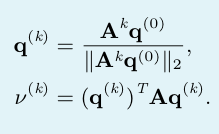
\includegraphics[scale =0.6 ]{./power_method.png}\\

\item [Shifted QR Method:] Basically, shifted QR is very similar to QR but we shift the diagonal of $A$ by $\mu$ before QR decomposition and shift it back after QR decomposition. \\
%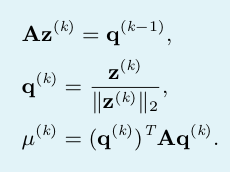
\includegraphics[scale =0.6 ]{./inverse_power.png}\\

\item [Error check:] I wrote a function QRerror() to check the error. The function is to check the largest magnitude of the elements just below the diagonal. When it becomes smaller than $tol$, which is set as $10^{-9}$, the function would terminate.\\
%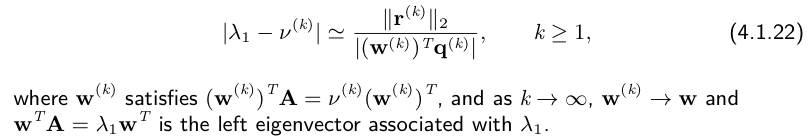
\includegraphics[scale =0.6 ]{./stopping_criteria.png}\\

\end{description}

\section{Workflow}

\begin{description}  

\item [Usage:] For example, time ./hw08.out < m3.dat
\item [Solve:] Use either shifted QR or QR to get the eigenvalues of $A$. Users should manually modify my code to use QR or shifted QR, default is set to QR.
\item[Desired output format:] The program shall print out on the screen the largest and smallest 3 eigenvalues and finally the iterations to reach error check.
\end{description}

\section{Results}

\begin{tabular}{|c|c|c|c|c|c|c|c|c|c|}
\hline  Matrix Dimension & Iterations\footnotemark[1] & CPU Time(s)\footnotemark[1]  & $\lambda_1$ & $\lambda_2$& $\lambda_3$  \\
\hline 3	&17/20	        &0/0	        		&6.372281	&2			&0.627719	\\
\hline 10	&35/249	        &0.005/0.012	&67.840399	&20.431729	&4.455992	\\
\hline 20	&67/909	        &0.021/0.256	&270.495189	&81.223819	&17.235222	\\
\hline 30	&107/1939	&0.099/1.793	&608.253606	&182.544889	&38.53868	\\
\hline 40	&137/3262	&0.282/7.379	&1081.115447	&324.394506	&68.364136	\\
\hline 50	&50000/4974	&212.621/22.997 &1689.080688	&506.772618	&106.711318	\\\hline

\end{tabular}
\begin{tabular}{|c|c|c|c|c|}
\hline   $\lambda_n$ & $\lambda_{n-1}$ & $\lambda_{n-2}$& Error\footnotemark[1]  \\
\hline 0.627719	&2			&6.372281	&4.79E-10/4.90E-10\\
\hline 0.512543	&0.55164		&0.629808	&8.96E-10/9.39E-10\\
\hline 0.503097	&0.512479	&0.528819	&9.75E-10/9.94E-10\\
\hline 0.501373	&0.505511	&0.512543	&8.00E-10/9.94E-10\\
\hline 0.500772	&0.503096	&0.507004	&9.86E-10/9.97E-10\\
\hline 0.499039/0.500494\footnotemark[1] 	&0.501061/0.501978	\footnotemark[1] &0.504326/0.500468	\footnotemark[1] &5.57E-3/9.97E-10\\\hline

\end{tabular}
\footnotetext[1]{The value to the left of slash is of Shifted QR Method, to the right is of QR Method}
\newpage
\section{Plot Analysis}
Both loglog plot and semi-log plot are provided.\\
1. Time\\
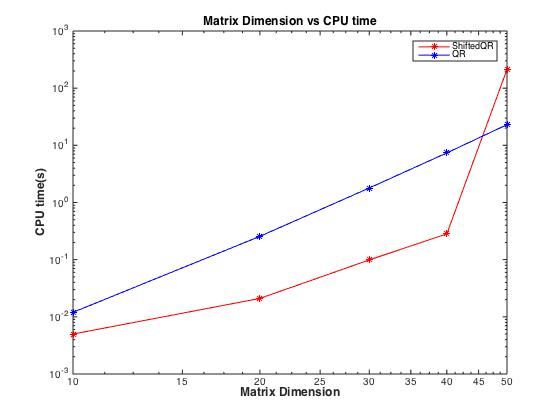
\includegraphics[scale =0.7 ]{./time.jpg}\\
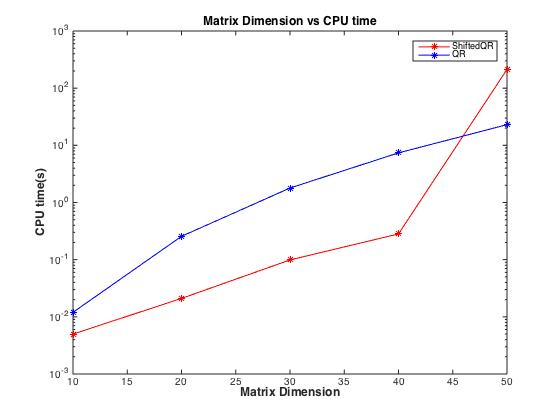
\includegraphics[scale =0.7]{./semitime.jpg}\\

2. Eigenvalues\\
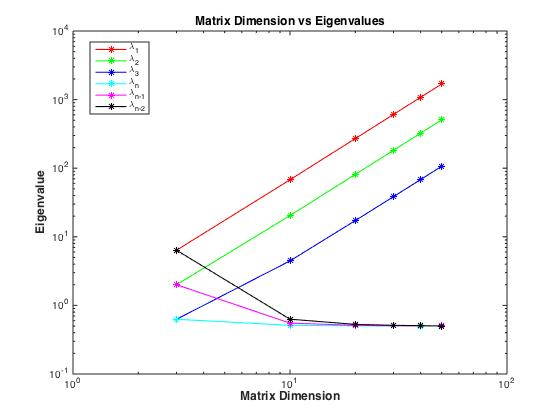
\includegraphics[scale =0.7]{./eig.jpg}\\
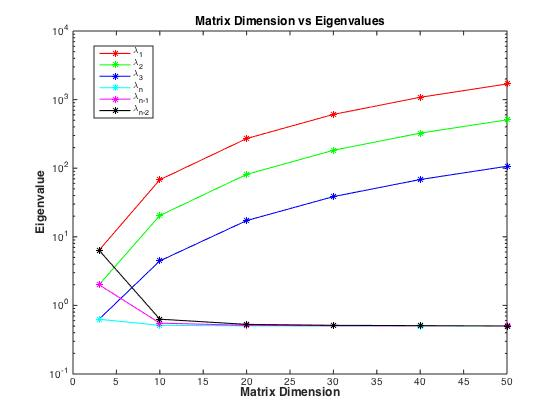
\includegraphics[scale =0.7]{./semieig.jpg}\\
\newpage
3. Iterations\\
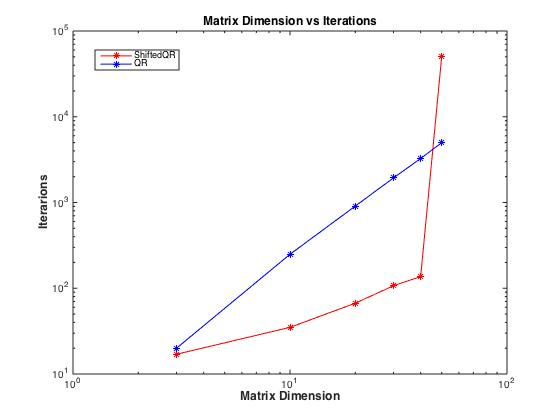
\includegraphics[scale =0.7]{./iter.jpg}\\
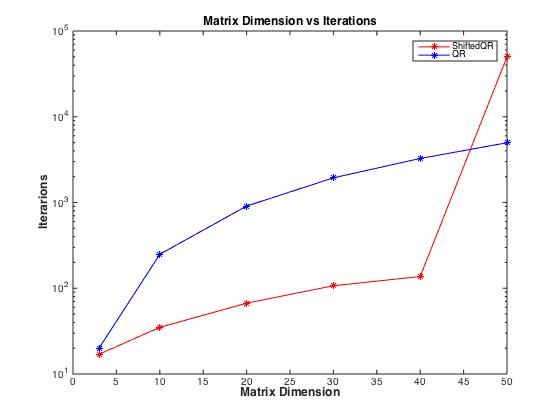
\includegraphics[scale =0.7]{./semiiter.jpg}\\
\section{Observations}

\begin{description}
\item [Notice:] When doing shifted QR on m8.dat, the method did NOT converge in the end, that is, the function would terminate before it reaches the error requirement. Definitely we can adjust the $maxIter$ to see if it can converge but it is not worth it to do that since the time already exceeds the time of QR. The reason could be that the $\lambda_n$ is too close to 0.5, so if we shift by 0.5, the matrix after QR decomposition will not converge. But, view from the data, the result of using shifted QR are still close to the real one.
\item [CPU time:]  The complexity of QR is approximately $O(n^5)$, to be specific, $O(n^{4.9177})$, derived from $\frac{log(7.379) - log(1.793)}{log(40) - log(30)}$, while the complexity of shifted QR is $O(n^{3.6387})$, derived from $\frac{log(0.282) - log(0.099)}{log(40) - log(30)}$. But the CPU time depends on the number of iteration, so we can only say that if the matrix expands with the same pattern, the complexity could be like the numbers above. It is not proper to judge the complexity of QR and shifted QR from data retrieved from this assignment. Notice: when calculating complexity, I omit the data point of shifted QR when dimension is 50.
\item [Eigenvalues:] Obviously, the smallest three eigenvalues tend to converge if the input matrix expands with the same pattern. Interestingly, the largest three eigenvalues all tend to grow quadratically, derived from $\frac{log(1081.115) - log(608.253)}{log(40) - log(30)}$ and so on. 

\item [Iteration:] The iteration for QR seems to grow exponentially with the exponent of roughly $1.8$, calculated from $\frac{(log(3262) - log(1939))}{(log(40) - log(30))}$. But I do not think I can do the same thing to shifted QR since the growing line is not as stable as QR is.

\item [Accuracy:]  I check all the biggest elements below the diagonal for $R * Q$ in each iteration. If even the biggest ones are still smaller than $10^{-9}$, the others will be even smaller. Therefore, my results are extremely close to the true eigenvalues.\\
%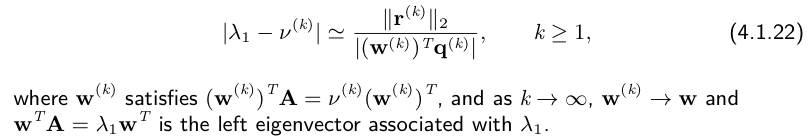
\includegraphics[scale =0.5]{./stopping_criteria.png}\\

\item[Overall:] The shifted QR is overall better than the QR but if one of the eigenvalues were close to the shifted value, it would be improper to use shifted QR. I suggest use inverse power method to find the smallest eigenvalue then we can decide what $\mu$ should be taken.

\end{description}


\end{document} 
